\documentclass[../main]{subfiles}
\usepackage{glossaries}

\begin{document}

\chapter{The \tested{} educational test framework}\label{ch:tested1}

We begin the chapter by giving a brief introduction and consider some related work.
Then, we look at the architectural design of the TESTed framework.
We then consider the three parts of evaluating a submission:
the test suite, the evaluation process itself, and the generated feedback:

\begin{itemize}
    \item For the test suites, we discuss their structure, although a user-friendlier format for test suites is TESTed-DSL (\vref{ch:tested-dsl}).
          We also look at how TESTed handles datatypes (of different programming languages) and statements or expressions.
    \item Next, the evaluation process is discussed in detail.
          This is the process through which TESTed executes the test suite and determines the feedback that will be given on the submission.
          This the meat of the chapter.
    \item We also briefly look at the integration with Dodona.
          This is relevant, as TESTed inherits some aspects from Dodona, such as the feedback format.
\end{itemize}

Afterwards, we describe how support for multiple programming languages is achieved.
We look at the internal API to give a good idea of what is required to support new programming languages.
Finally, we evaluate TESTed in educational practice.

\section{Introduction and background}\label{sec:tested1-introduction-and-background}

Formative feedback on solutions for programming exercises is a crucial part of learning to code~\autocite{shuteFocusFormativeFeedback2008,orrellFeedbackLearningAchievement2006,luxton-reillyIntroductoryProgrammingSystematic2018}.
Feedback is formative (and most valuable) if learners receive rich and qualitative feedback throughout the learning process.
Providing such feedback by hand is a challenge for educators since it is a time-consuming activity~\autocite{camposMultinationalCaseStudy2012,cheangAutomatedGradingProgramming2003, keuningSystematicLiteratureReview2018,haoUnderstandingEffectiveDesign2021,zavalaUseSemanticBasedAIG2018,staubitzRepositoryOpenAutogradable2017,pirttinenCrowdsourcingProgrammingAssignments2018,gulwaniFeedbackGenerationPerformance2014,tangDataDrivenTestCase2016,edwardsDevelopingCommonFormat2008a}.
The challenge is further exacerbated by a large number of students who work on multiple exercises~\autocite{campGenerationCSGrowth2017,saxExaminingEnrollmentGrowth2017}.
Any laborious and time-consuming activity is a prime target for automation, and providing feedback is no different.
The computer science education field therefore has a long history of applying software test frameworks or general-purpose software tools (linters, formatters, etc.) on source code to automatically generate feedback~\autocite{haoUnderstandingEffectiveDesign2021,edwardsUsingSoftwareTesting2004,paivaAutomatedAssessmentComputer2022a,keuningSystematicLiteratureReview2018}.

Off-the-shelf tools such as linters are low effort for educators, but only provide generic feedback: there is no exercise-specific feedback.
Software testing frameworks require an accompanying test suite for each individual programming exercise, but can provide much more specific feedback.
A test suite typically contains a set of tests that verify if the submission satisfies the requirements in the problem statement of the exercise.
This is similar to the practice of unit tests or integration tests in the software engineering field.
Beside general testing frameworks, computer science education also uses judge systems~\autocite{paivaAutomatedAssessmentComputer2022a,wasikSurveyOnlineJudge2018}: specialized learning environments that provide rich feedback.
Defining an adequate test suite for an exercise is part of the reason why creating programming exercises is so time-consuming~\autocite{zavalaUseSemanticBasedAIG2018,staubitzRepositoryOpenAutogradable2017,queirosPexilProgrammingExercises2011,pirttinenCrowdsourcingProgrammingAssignments2018,gulwaniFeedbackGenerationPerformance2014,tangDataDrivenTestCase2016}.

An apparent solution to reduce the amount of time needed to create programming exercises is to create fewer exercises.
To achieve this without reducing the number of exercises available to students, maximal reuse of existing exercises is necessary.
Existing solutions to facilitate reusing exercises include standard formats in which exercises are written~\autocite{paivaAnotherProgrammingExercises2020,verhoeffProgrammingTaskPackages2008}, open repositories with exercises~\autocite{staubitzRepositoryOpenAutogradable2017}, or tools to convert between existing exercise formats~\autocite{queirosBabeLOExtensibleConverter2013}.
However, reusing exercises remains difficult, particularly when attempting to reuse exercises across programming languages.
In existing judge systems, exercises are tightly coupled to the programming language in which the test suite is written.
Alternatively, test suites without such a tight coupling impose stringent restrictions on exercise specifications, e.g.\ only reading from stdin and writing to stdout.
Because of these restrictions, they often generate feedback of a lower quality than programming-language specific test suites.

To reuse programming exercises written for another programming language, exercise designers first have to learn a new test framework for that programming language.
Then, they have to write a new test suite for the exercise according to the specifications of the new test framework.
Alternatively, due to the vast number of programming languages~\autocite{bissyandePopularityInteroperabilityImpact2013}, it might be necessary to implement a new test framework to support educational software testing, which is no small undertaking.

We focus on facilitating easy reuse of programming exercises across programming languages.
Our contributions include defining requirements for a test framework to support multiple programming languages, without imposing strict restrictions on programming exercises.
We also introduce TESTed, a proof-of-concept of a system that satisfies these requirements.
TESTed directly supports multiple programming languages for the same exercise, meaning the conversion of exercises to multiple test frameworks is no longer needed.
Exercise designers working on exercises for a single programming language can also benefit from TESTed, as it no longer forces them to learn new test frameworks for each new target language.
Finally, implementing support for new programming languages in TESTed is less work than implementing a complete test framework for each individual language, reducing the software development and maintenance cost dramatically.

\section{Related work}\label{sec:tested1-related-work}

Since the terminology related to automated feedback on programming exercises is not used consistently within the field,
we begin by defining the terms used in this manuscript.
A programming exercise is the combination of a \textbf{problem statement} and a \textbf{test suite}.
When students attempt to solve the exercise using the instructions from the problem statement, they create a \textbf{submission} for the exercise.
The test suite is used by a judge system to \textbf{evaluate} the submission.
This results in \textbf{feedback} that is shown to the student.

We consider it useful to split a judge system into a \textbf{judge platform} and a \textbf{test framework}.
A judge platform is the graphical user interface that allows students and educators to upload and store submissions, display feedback, organize exercises into courses, and so on.
A test framework is responsible for generating feedback, by executing and evaluating submissions based on an exercise-specific test suite.
In existing literature, the distinction between these two is not always made, nor is it always relevant.
For example, some review manuscripts~\autocite{keuningSystematicLiteratureReview2018,wasikSurveyOnlineJudge2018} or individual tools~\autocite{bezURIOnlineJudge2014,petitJutgeOrgCharacteristics2018} consider the entire system as a whole.
Other manuscripts focus specifically on judge platforms~\autocite{gusukumaPedalInfrastructureAutomated2020,strieweArchitectureModularGrading2016}.
However, we believe this distinction is relevant for this manuscript, as evaluating submissions (the test framework) has a separate set of challenges compared to judge platforms (e.g.\ displaying feedback in a constructive way).
This manuscript focuses on test frameworks.

In educational contexts, software testing frameworks typically use either \textbf{output comparison} or \textbf{unit testing}~\autocite{paivaAutomatedAssessmentComputer2022a} to evaluate submissions.
Programming language support of test frameworks generally depends on the approach they adopt.
With unit testing, the test suite is often written in the same programming language as the submission, e.g.\ with tools based on xUnit~\autocite{meszarosXUnitTestPatterns2007}.
Since the test suite is often written in the same programming language as the submission, it has full access to the submission.
The test suite can use function calls, data structures (e.g.\ lists, maps), primitive data types (e.g.\ integers, strings), examine return values, exceptions, runtime inspections (e.g.\ reflection), etc.
As a result, the test suite is tightly coupled to a specific programming language.
Evaluating a submission for the same exercise in another programming language would require a new test suite, often also involving another test framework.

With output comparison, the judge system imposes stringent restrictions on the programming exercise: only stdin, stdout, stderr and files can be used for input and output.
Prominent examples are the test frameworks used in ICPC-style (\emph{International Collegiate Programming Contest}, sometimes still referred to as ACM-ICPC)~\autocite{ICPCFactSheet2020} programming contests.
While this approach makes test suites independent of any programming language, the restrictions yield that testing is limited to data passed through stdin/stdout/stderr or via files.
All aspects of the submission that the test suite needs to check must be converted to a textual representation.
Files can contain binary data, but the same limitations apply.
Another disadvantage is the lack of granular testing: with these systems, tests are limited to the program as a whole.
It is, for example, not possible to add distinct tests for different functions inside the same program without obligating students to artificially split the program.

\section{Programming-language-agnostic test frameworks}\label{sec:tested1-programming-language-agnostic-test-frameworks}

Intuitively, an ideal test framework that supports multiple programming languages is a test framework with the testing capabilities of unit testing and the programming language support of output comparison.
First, we define the two requirements a framework needs to satisfy to achieve this.
We also look at the consequences of those requirements on the framework.
We call a test framework that satisfies these requirements a \emph{programming-language-agnostic test framework}.

The \textbf{first requirement} is that test suites must be programming language independent.
A test suite must be usable to evaluate submissions in every programming language supported by the framework, without making changes to the test suite or adding languages-specific tests to it.
As a consequence of this requirement, adding support for new programming languages to the test framework must not demand changes to existing test suites.
All existing test suites must work with the new programming language without changes.

The \textbf{second requirement} is similar testing capabilities as unit testing.
Some concrete examples of what should be possible are:

\begin{itemize}[noitemsep]
    \item Provide textual input to stdin and reading output from stdout.
    \item Call functions implemented in submissions, and pass arguments to those functions.
    \item Evaluate values returned from function calls (with data type support).
    \item Create objects (constructors) and manipulate them (methods).
    \item Capture and evaluate other side effects such as exceptions, exit codes or files (or other persistent storage such as databases).
    \item Support exercises with deterministic/non-deterministic (e.g.\ random) behavior.
\end{itemize}

Support for these two requirements should not have disproportionately large drawbacks.
Therefore, we also consider the following soft requirements for a programming-language-agnostic test framework:

\begin{itemize}
    \item Configuring or creating exercises using the framework should not be significantly more difficult than configuring exercises using a language-specific test framework.
    \item Runtime and memory overhead should be minimal: the framework cannot be unacceptably slow or have a large memory footprint compared to a language-specific test framework.
    Providing feedback to students in a timely manner is important.
    \item Submissions should follow their language-specific conventions as closely as possible.
    For example, we want to support asynchronous and synchronous functions in JavaScript, or top-level functions should be implemented as a static function in Java, but not in Python or Kotlin that have proper support for top-level functions.
    \item Adding support for new programming languages to the framework should ideally be faster than implementing language-specific test frameworks for those languages, due to the ability to reuse shared parts of the implementation.
\end{itemize}

\section{Using the framework}\label{sec:tested1-using-the-framework}

We start with a high-level tour of TESTed, focussing on how the framework can be used.
To this end, we will use the following programming exercise as an example:

\begin{quote}
    Implement a function \texttt{remove\_all\_occurrences} that takes two arguments: a list $l$ of integers and an integer $v$.
    The function must return a new list containing the same integers as list $l$, in the same order, but where all occurrences of integer $v$ are removed.
\end{quote}

A correct Python implementation for this exercise could be:

\begin{minted}{python}
def remove_all_occurrences(l, v):
    return [x for x in l if x != v]
\end{minted}

A test suite for this exercise could contain a number of function calls with different arguments and check their return values against an expected value.
To keep things short, we limit ourselves here to a test suite with a single function call (\cref{lst:simple-json-test-suite}).

\begin{listing}
    \begin{minted}{json}
{
 "input": {
  "type": "function",
  "name": "remove_all_occurrences",
  "arguments": [
   {
    "type": "sequence",
    "data": [
     {"data": 1, "type": "integer"},
     {"data": 2, "type": "integer"},
     {"data": 3, "type": "integer"},
     {"data": 2, "type": "integer"}
    ]
   },
   {"data": 2, "type": "integer"}
  ]
 },
 "output": {
  "result": {
   "type": "sequence",
   "data": [
    {"data": 1, "type": "integer"},
    {"data": 3, "type": "integer"}
   ]
  }
 }
}
    \end{minted}
    \caption[]{
        Snippet of a JSON test suite for with a single test case that calls the function \mintinline{python}{remove_all_occurrences} with two arguments:
        \begin{enumerate*}[label=\emph{\roman*})]
            \item a sequence containing the four integers 1, 2, 3 and 2,
            \item the integer 2.
        \end{enumerate*}
        The expected return value is a list containing the integers 1 and 3.
    }
    \label{lst:simple-json-test-suite}
\end{listing}

When evaluating a submission using this test suite, TESTed will first translate the test suite into the programming language of the submission.
Conceptually, each function call is converted into a test case:

\begin{minted}{python}
# Python
remove_all_occurrences([1, 2, 3, 2], 2) == [1, 3]
\end{minted}

\begin{minted}{javascript}
// JavaScript
removeAllOccurrences([1, 2, 3, 2], 2) === [1, 3]
\end{minted}

\begin{minted}{haskell}
-- Haskell
(removeAllOccurrences [1, 2, 3, 2] 2) == [1, 3]
\end{minted}

TESTed takes care of the differences between programming languages (e.g.\ syntax, default representations and naming conventions).
The actual test code generated by TESTed is more complex, as it must capture return values, account for exceptions, etc.

When TESTed evaluates the correct Python submission from above, it produces the following Python-specific feedback:

\begin{minted}{json}
{"command": "start-testcase"}
{"description": "remove_all_occurrences([1, 2, 3, 2], 2)"}
{"expected": "[1, 3]", "channel": "return"}
{"generated": "[1, 3]", "status": "correct"}
{"command": "close-testcase"}
\end{minted}

A judge platform may then use this output to display a human-readable representation of the feedback (an example of this can be seen in \vref{fig:dodona}.
The feedback starts with a description of what has been tested (a function call in the programming language of the submission, in this case Python), followed by the expected return value and the actual return value (in a human-readable string representation).
With the actual return value, a decision is also given: in this case, the return value is correct.

While the output for correct submissions is important, the output for wrong submissions is at least as important in the context of an educational test framework.
Assume a submission is wrong in that it only removes the first occurrence of the integer $v$ from the list $l$ (example in JavaScript):


\begin{minted}{javascript}
function removeAllOccurrences(l, v) {
  l.splice(l.indexOf(v), 1);
  return l;
}
\end{minted}

When TESTed evaluates this submission, its feedback reflects that while the code has been executed successfully, a logical error was found:

\begin{minted}{json}
{"description": "removeAllOccurrences([1, 2, 3, 2], 2)"}
{"expected": "[1, 3]", "channel": "return"}
{"generated": "[1, 3, 2]", "status": "wrong"}
\end{minted}

However, students sometimes do not even get to the point where their submission is executed successfully.
For example, they might submit a solution containing a syntax error (in Python):

\begin{minted}{json}
{"description": "remove_all_occurrences([1, 2, 2, 3], 2)"}
{"message": "Received compiler error:"}
{"message": "*** Error compiling..." }
{"status": "compilation error"}
\end{minted}

Instead of an expected and actual return value, the feedback now contains the error message printed by the Python compiler (using \mintinline{console}{python -m compileall}).
If compilation fails, the submission will not be executed and testing is stopped.

\section{Architectural design of the framework}\label{sec:tested1-architectural-design}

\begin{figure}[t]
    \centering
    \includestandalone{concept}
    \caption{
        Architectural design of TESTed, with colors indicating different programming languages.
        The framework consists of a set of Python packages and modules.
        These can be categorized as the core package and a set of programming-language-specific modules.
        The input for TESTed consists of a test suite, together with a submission in one of the supported programming languages.
        The output is the generated feedback.
    }
    \label{fig:conceptual-design}
\end{figure}

TESTed is built around the idea that an exercise author writes a single, unified test suite for the exercise, independent of any programming language.
TESTed then converts that test suite into the programming language of the submission on the fly, and takes care of the various aspects of the evaluation process: compile the submitted code, execute the submission together with the test code, check test results, and generate feedback.

While some parts of the evaluation process are programming-language-specific by necessity, such as generating the test code, a lot of the steps are not.
For example, creating an execution plan or interpreting the test results and generating the feedback are not specific to any one programming language.
Therefore, the language-specific aspects are isolated in language modules, as illustrated in~\vref{fig:conceptual-design}.

\leavevmode\marginnote{
    A Python module is a \texttt{.py} file, while a Python package is a folder containing modules.
}%
TESTed is written in Python and organized into a set of Python modules and packages.
An import package is the \emph{core} package, which contains modules that are responsible for all language-independent tasks, such as scheduling tests.
We provide an in-depth description of the full evaluating process in \cref{subsec:execution-planning}.
In most cases, the core is also responsible for checking the collected test results and generating the feedback.
This is discussed in \cref{subsec:checking-results}.

All aspects that are specific to one programming language are bundled in one package.
These language-specific modules take care of all language-specific tasks, such as compiling submissions, executing submissions, and handling language-specific data types, expressions, and statements.
Since the language-specific code is limited to these modules, this offers benefits for adding support for new programming languages to TESTed, see \vref{sec:programming-language-support}.

TESTed takes as input the test suite for a programming exercise and a possible solution that needs to be evaluated.
The format of the test suite is discussed in-depth in (\cref{sec:test-suites}).
As a result of its evaluation, TESTed outputs a feedback report (\cref{sec:tested-and-dodona})

\section{Test suites}\label{sec:test-suites}

Despite multiple proposals on generic formats for programming exercises~\autocite{edwardsDevelopingCommonFormat2008a,paivaAnotherProgrammingExercises2020,queirosPexilProgrammingExercises2011,verhoeffProgrammingTaskPackages2008} or exercise classifications~\autocite{leOperationalizingContinuumWellDefined2013,simoesNatureProgrammingExercises2020}, there seems to be no generally accepted standard for test suites of programming exercises.
Additionally, none of the proposed formats meets the requirements that we identified for language-agnostic test frameworks.
Existing formats focus mostly on the description of the problem statement, whereas we also focus on the specification of the test suite itself.

We therefore feel it is appropriate to introduce a new format for test suites, specifically developed for TESTed.
It is designed to be machine and human-readable and easy to generate.
Making it ergonomic to write by hand was only a secondary goal.
While the format is not framework specific, and could thus be adopted by other test frameworks, this was not an explicit design goal.

Test suites for TESTed are written in JSON, which was chosen because there is broad support in programming languages.
Additionally, it is human editable and readable, especially compared to binary formats.
There is also widespread editor support for JSON, and technologies such as JSON Schema allow for easy validation and even better editor support.

These test suites are a direct JSON representation of the internal structure of a test suite as used by TESTed.
While JSON test suites have some advantages, such as being more flexible in some ways, they are also much more verbose and not guaranteed to stay stable.
Being a representation of the internal structure, no processing is done: the test suite must be fully ``rolled out''.
For example, only the lowest levels of the test suite (the tests) can have options in the JSON suite.

Note that TESTed-DSL (\vref{ch:tested-dsl}) is the intended way for exercise authors to create exercises, especially if done manually.

\subsection{Structure of a test suite}\label{subsec:structure-of-a-test-suite}

\begin{listing}
    \begin{minted}{json}
{
 "variable": "a_list",
 "type": "sequence",
 "expression": {
  "type": "sequence",
  "data": [
   {"data": 1, "type": "integer"},
   {"data": 2, "type": "integer"},
   {"data": 3, "type": "integer"},
   {"data": 2, "type": "integer"}
  ]
 }
}, {
 "input": {
  "type": "function",
  "name": "remove_all_occurences",
  "arguments": [
   "a_list",
   {"data": 2, "type": "integer"}
  ]
 },
 "output": {
  "result": {
   "value": {
    "type": "sequence",
    "data": [
     {"data": 1, "type": "integer"},
     {"data": 3, "type": "integer"}
    ]
   }
  }
 }
}
    \end{minted}
    \caption[]{
        A snippet of a JSON test suite for TESTed with two statements:
        \begin{enumerate*}[label=\emph{\roman*})]
            \item declaration of a variable (\texttt{aList}) that is assigned a sequence containing four integers 1, 2, 3, and 2 and
            \item call of the function \texttt{remove\_all\_occurrences} with two arguments: \texttt{aList} and the integer 2.
        \end{enumerate*}
        The expected return value is a list containing the integers 1 and 3.
    }
    \label{lst:expanded-json-fragment}
\end{listing}

Returning to the sample programming exercise we used before, we can expand the test suite (\vref{lst:simple-json-test-suite}) for illustration purposes (\cref{lst:expanded-json-fragment}).
Instead of directly calling the function \mintinline{python}{remove_all_occurrences} with two arguments, we first create a list and assign it to a variable in the first test case.
In the second test case, we then call the function \mintinline{python}{remove_all_occurrences}, but use the variable name as the first argument.

While omitted for brevity in the examples, a test suite can organize test cases in two levels: tabs and contexts.
The full hierarchy of the test suite thus consists of four levels, from top to bottom (\vref{fig:dodona}):

\begin{enumerate}
    \item \textbf{Tabs} are the top-level grouping mechanism.
          It allows logically grouping contexts together.
          While the name of this group suggests how to display these groups, it is but a suggestion.
          The example only has one tab, but a test suite with test cases for multiple functions might for example have one tab per function.
    \item \textbf{Contexts} are meant to group dependent test cases together.
          In our example, declaring a variable and using that variable must be done within the same context.
    \item \textbf{Test cases} are the basic building blocks of the test suite.
          The ``input'' for a test case is what exactly is being checked.
          For example, text via stdin, a function call or an expression.
          In the example, the first test case of each context has an assignment, while the second has a function call.
    \item \textbf{Tests} are used for each type of output.
          TESTed currently supports return values, standard output (stdout), standard error (stderr), exceptions, generated files and exit codes.
          In the example there is one test for the return value.
          If a test is not defined (e.g.\ for stderr in the example), a sensible default is used.
          For example, the default test for stdout and stderr checks that there is no output, causing the evaluation to fail if there is unexpected output.
\end{enumerate}

This structure mirrors the output generated by TESTed (\vref{sec:tested-and-dodona}).
For example, the executed input for each test is also included in the output.
A possible visualization of these levels is given in \vref{fig:dodona}, which shows the output rendered in Dodona~\autocite{vanpetegemDodonaLearnCode2023}.

Note that in this manuscript, we use the Dodona naming scheme for the test hierarchy.
TESTed also supports an alternative, which is more in line with the terminology used in the literature: tabs, contexts, testcases, and tests are called \textbf{units}, \textbf{testcases}, \textbf{tests}, and \textbf{scripts} respectively.

\begin{figure}
    \centering
    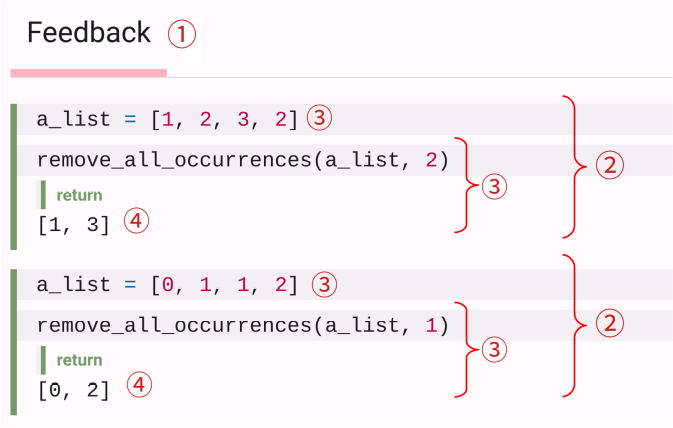
\includegraphics[width=0.8\textwidth]{dodona-rendering}
    \caption{A way to visually render the feedback (as done in Dodona) resulting from evaluating a submission (in Python) with the test suite from \vref{lst:expanded-json-fragment}.
    There are four levels: \CircledText{1} tabs, \CircledText{2} contexts, \CircledText{3} units, and \CircledText{4} the tests.
    Here, each context consists of two testcases, the first of which has no tests, while the second has one test (the expected return value).}
    \label{fig:dodona}
\end{figure}

\subsection{Data serialization}\label{subsec:data-serialization}

TESTed uses data serialization to convert between the language-independent format of the test suite, and the generated test code.
Additionally, the same data serialization is used to convert return values from the submission into the language-independent format for checking (as described in \vref{subsec:checking-results}).

\begin{table}
    \caption{
        Overview of the basic types of TESTed and their implementation in the programming languages supported by TESTed.
        Sometimes, another type is used instead, based on the value. For example, an integer that is too large for \texttt{int} in Java will become a \texttt{long}.
        A dash (-) is used to indicate that the programming language does not support this type.
    }
    \label{tab:tested-basic-types}
    \begin{wide}
        \small\setlength{\tabcolsep}{0.25\tabcolsep}%
        \begin{tabular}{|l|l|l|l|l|l|l|l|l|}
            \hline
            \tested{} & Python         & JavaScript       & Java             & Kotlin           & Haskell          & C               & Bash          & C\#                 \\
            \hline
            integer   & \texttt{int}   & \texttt{number}  & \texttt{int}     & \texttt{Int}     & \texttt{Int}     & \texttt{int}    & -             & \texttt{Int32}      \\
            real      & \texttt{float} & \texttt{number}  & \texttt{double}  & \texttt{Double}  & \texttt{Double}  & \texttt{double} & -             & \texttt{Double}     \\
            boolean   & \texttt{bool}  & \texttt{boolean} & \texttt{boolean} & \texttt{Boolean} & \texttt{Bool}    & \texttt{bool}   & -             & \texttt{Boolean}    \\
            text      & \texttt{str}   & \texttt{String}  & \texttt{String}  & \texttt{String}  & \texttt{String}  & \texttt{char*}  & \texttt{text} & \texttt{string}     \\
            sequence  & \texttt{list}  & \texttt{array}   & \texttt{List}    & \texttt{List}    & \texttt{{[}{]}}  & -               & -             & \texttt{List}       \\
            set       & \texttt{set}   & \texttt{Set}     & \texttt{Set}     & \texttt{Set}     & -                & -               & -             & \texttt{Set}        \\
            map       & \texttt{dict}  & \texttt{object}  & \texttt{Map}     & \texttt{Map}     & -                & -               & -             & \texttt{Dictionary} \\
            nothing   & \texttt{None}  & \texttt{null}    & \texttt{null}    & \texttt{null}    & \texttt{Nothing} & \texttt{void}   & -             & \texttt{void}       \\
            \hline
        \end{tabular}
    \end{wide}
\end{table}

Each literal value is described by an object with two attributes: a value (e.g.\ the number \texttt{5.3}) and a data type (e.g.\ \texttt{real}).
These attributes are combined into a JSON object with two fields.
The value is encoded using the closest representation available in JSON\@.
For example, a number is represented by a JSON number, and a string is represented by a JSON string.
The data type of a literal value is more complex, since TESTed targets multiple programming languages that each support their own collection of data types.
TESTed therefore defines a set of rules to denote data types and their support in programming languages.
This allows TESTed to convert types between programming languages.

TESTed uses two categories of data types.
The first category is a limited set of \textbf{basic types} that are abstract and map to concepts.
Currently, the following basic types are supported:

\begin{description}[noitemsep]
    \item[\texttt{integer}] An integer. The size of the integer is left undefined.
    \item[\texttt{real}] A real number. The size and precision of the real is left undefined.
    \item[\texttt{boolean}] A Boolean value.
    \item[\texttt{text}] Textual data (e.g.\ strings).
          The intention is important here: for example, an ASCII character can be represented as both an integer or as text.
    \item[\texttt{sequence}] An ordered sequence of values.
    \item[\texttt{set}] An unordered collection of unique values.
    \item[\texttt{map}] A collection of key-value pairs, where the keys are unique.
    \item[\texttt{nothing}] A representation of ``nothing'', meaning no value. \marginnote{The \texttt{any} type acts roughly as the \emph{top type}, except that we do not have a formal type system, nor do we have subtypes.}
    \item[\texttt{any}] Any or unknown data type.
         This type is not usable in test suites, but is used to indicated return values of an unknown type.
\end{description}

When a test suite contains a literal value of a basic type, it will be serialized as an object of an actual data type in the target programming language.
An overview of all basic types and their implementation is given in \vref{tab:tested-basic-types}.
For example, a literal value with data type \texttt{map} will become a \texttt{Map} in Java or a \texttt{dict} in Python.

The second category consists of \textbf{advanced types}, which are more detailed or programming language specific.
Each advanced type is associated with a basic type, acting as a fallback.
For example, \texttt{int64} is an advanced type with the basic type \texttt{integer} as a fallback.
If a programming language does not support a particular advanced type, the corresponding basic type will be used.
For example, consider tuples.
Many programming languages do not have direct support for tuples, but exercises using tuples can still be solved by using the corresponding basic type (sequence).
For a concrete example, an exercise using a \texttt{tuple} can be solved in Java by using a \texttt{List}.

When adding a programming language, it is possible to disable this fallback for certain types.
For example, JavaScript has no support for fixed precision numbers.
This prevents TESTed from evaluating submissions in JavaScript if fixed precision numbers are used in the test suite.
TESTed will generate an appropriate error in this case.

Currently supported advanced types are:

\begin{description}[noitemsep]
    \item[\texttt{int8}] 8-bit integers (signed)
    \item[\texttt{uint8}] 8-bit natural numbers (unsigned)
    \item[\texttt{int16}] 16-bit integers (signed)
    \item[\texttt{uint16}] 16-bit natural numbers (unsigned)
    \item[\texttt{int32}] 32-bit integers (signed)
    \item[\texttt{uint32}] 32-bit natural numbers (unsigned)
    \item[\texttt{int64}] 64-bit integers (signed)
    \item[\texttt{uint64}] 64-bit natural numbers (unsigned)
    \item[\texttt{bigint}] integers without upper and lower limit (signed)
    \item[\texttt{single\_precision}] single precision real number
    \marginnote{The names for real numbers are borrowed from IEEE 754.}
    \item[\texttt{double\_precision}] double precision real number
    \item[\texttt{double\_extended}] double extended precision real number
    \item[\texttt{fixed\_precision}] fixed precision real number
    \item[\texttt{array}] a mutable fixed-size sequence
    \item[\texttt{list}] a mutable variable-size sequence
    \item[\texttt{tuple}] an immutable sequence
    \item[\texttt{char}] a single character
    \item[\texttt{undefined}] \texttt{undefined} in JavaScript
    \item[\texttt{null}] \texttt{null} in JavaScript
\end{description}

The advanced data types are also where the language-specific aspects can come into play.
For example, in addition to the basic type \texttt{nothing}, we have both \texttt{undefined} and \texttt{null}.
In most languages, there is no difference between those, but for example, in JavaScript there is.
Having both available as an advanced type allows exercises to use either in JavaScript exercises, while still being language-agnostic.

% TODO: move to appendix
%An overview of the supported advanced types for each programming language is given in \cref{tab:tested-advanced-types}.
%A plus sign (+) in a column indicates that the programming language has limited support for the data type.
%This means that the programming language will fall back to the basic type (as discussed previously).
%A dash means there is no support in the programming language: exercises using this data type will not be solvable in that programming language.

%\begin{table}
%    \caption{
%        An overview of advanced types supported by TESTed.
%        The first column contains all advanced types, and the second column contains their corresponding basic type.
%        The other columns contain the mapping to the data types of the programming languages currently supported.
%        Note that the table is split into two.
%    }
%    \begin{wide}
%        \small\setlength{\tabcolsep}{0.5\tabcolsep}%
%        \begin{tabular}{|l|l|l|l|l|l|l|l|l|}
%            \hline
%            \tested{}         & Basic & Python         & JavaScript       & Java             & Kotlin   \\
%            \hline
%            int8              & integer & + & + & \texttt{byte} & \texttt{Byte} \\
%            uint8             & integer & + & + & + & \texttt{UByte} \\
%            int16             & integer & + & + & \texttt{short} & \texttt{Short} \\
%            uint16 & integer & + & + & + & \texttt{UShort} \\
%            int32 & integer & + & + & \texttt{int} & \texttt{Int} \\
%            uint32 & integer & + & + & + & \texttt{UInt} \\
%            int64 & integer & + & + & \texttt{long} & \texttt{Long} \\
%            uint64 & integer  & + & + & + & \texttt{ULong} \\
%            bigint & integer  & \texttt{int} & \texttt{BigInt} & \texttt{BigInteger}
%            & \texttt{BigInteger} \\
%            single\_precision & real & + & + & \texttt{float} & \texttt{Float} \\
%            double\_precision & real & + & + & \texttt{double} & \texttt{Double} \\
%            double\_extended & real & + & + & + & + \\
%            fixed\_precision & rational & \texttt{Decimal} & - & \texttt{BigDecimal}
%            & \texttt{BigDecimal} \\
%            array & sequence & + & + & \texttt{array} & \texttt{Array} \\
%            list & sequence & \texttt{List} & + & \texttt{List} & \texttt{List} \\
%            tuple & sequence & \texttt{Tuple} & + & + & + \\
%            char & text & + & + & \texttt{char} & \texttt{Char} \\
%            undefined & nothing & + & \texttt{undefined} & + & + \\
%            \hline
%        \end{tabular}
%        \begin{tabular}{|l|l|l|l|l|l|l|l|l|}
%            \hline
%            \tested{}         & Haskell                   & C                        & Bash & C\# \\
%            \hline
%            int8              & \texttt{Data.Int.Int8}    & +                        & -    & \\
%            uint8             & \texttt{Data.Word.Word8}  & +                        & -    & \\
%            int16             & \texttt{Data.Int.Int16}   & \texttt{short}           & -    & \\
%            uint16            & \texttt{Data.Word.Word16} & \texttt{unsigned\ short} & -    & \\
%            int32             & \texttt{Data.Int.Int32}   & \texttt{int}             & -    & \\
%            uint32            & \texttt{Data.Word.Word32} & \texttt{unsigned\ int}   & -    & \\
%            int64             & \texttt{Data.Int.Int64}   & \texttt{long}            & -    & \\
%            uint64            & \texttt{Data.Word.Word64} & \texttt{unsigned\ long}  & -    & \\
%            bigint            & \texttt{Integer}          & -                        & -    & \\
%            single\_precision & \texttt{Float}            & \texttt{float}           & -    & \\
%            double\_precision & \texttt{Double}           & \texttt{double}          & -    & \\
%            double\_extended  & -                         & \texttt{double\ double}  & -    & \\
%            fixed\_precision  & -                         & -                        & -    & \\
%            array             & -                         & -                        & -    & \\
%            list              & \texttt{{[}{]}}           & -                        & -    & \\
%            tuple             & \texttt{()}               & -                        & -    & \\
%            char              & \texttt{Char}             & \texttt{char}            & +    & \\
%            undefined         & +                         & +                        & -    & \\
%            \hline
%        \end{tabular}
%    \end{wide}
%    \label{tab:tested-advanced-types}
%\end{table}

\subsection{Statements and expressions}\label{subsec:tested1-statements-and-expressions}

We return once more to the test suite from \vref{lst:simple-json-test-suite}, which evaluates a function call.
It illustrates the need for TESTed to support a language-independent description of expressions and statements.
Evaluation of an expression yields a value, where TESTed allows to describe expected values as identifiers (referring to a variable that was previously defined), function calls or literal values (using the data serialization format described in the previous section).
A statement in TESTed is either an assignment (defining a new variable) or an expression (similarly to Python: every expression on its own is also a statement).

Note the absence of control structures or operators in the description of expressions and statements.
Our goal is not to create a full-fledged abstract programming language.
We intentionally limit expressions and statements to features needed by TESTed.
Creating a universal programming language that can be converted to all other programming languages is out of scope.

The use of assignments is illustrated by the expanded test suite in \vref{lst:expanded-json-fragment}.
We create a list and assign it to a variable \texttt{a\_list}.
Note that there are no tests in this first test case.
The second test case then calls the function but uses the variable we defined as the first argument.

\section{Evaluating submissions}\label{sec:tested1-evaluating-submissions}

This section explains in detail the complete evaluation process that is performed when a submission is evaluated.
The input for the evaluation process is a test suite and a submission, which is typically provided by the judge platform in which TESTed runs (or can be provided manually if TESTed is run on the command line).
Subsequent subsections dive into more detail of individual parts of the process.

\Vref{fig:flow} is a schematic overview of said evaluation process.
The very first step in the evaluation process is checking if the exercise is solvable in the programming language of the submission (\cref{subsec:solvability-and-correctness-checks}).
Next, the test suite is partitioned into compilation and execution units (\cref{subsec:execution-planning}).
For each of these units, the relevant code is generated and the resulting test code is compiled (\cref{subsec:code-generation}).
This code is generated in the programming language of the submission.
This code generation is the bulk of language-specific code in TESTed, whose design and implementation are discussed in \vref{sec:programming-language-support}.

After compilation, each resulting executable contains one or more execution units.
These are then all executed, and the side effects (such as exceptions, stdout, stderr, etc.) and results (i.e.\ return values) are recorded (\cref{subsec:executing-test-code}).
These results are then checked for correctness against the test suite (\cref{subsec:checking-results}).
This results in the feedback, which is returned by TESTed.

TESTed also provides an opportunity for static analysis on the submission.
\marginnote{Examples include \software{ESLint}, \software{Pylint}, and \software{HLint}.}
Currently, all supported programming languages run a linter on the submission, the results of which are also included in the feedback as code annotations (\cref{subsec:static-analysis-of-the-submission}).

\begin{figure}
    \centering
    \includestandalone{flow}
    \caption{
        The process of evaluating a submission in TESTed.
        TESTed is typically run within a judge platform, which provides the submission, the test suite and the configuration options.
        The contexts in the test suite are organized into compilation units and then execution units.
        For each compilation unit, the test code is generated, which is then compiled.
        The execution units are then executed, which yields execution results. These are then checked, resulting in feedback.
        Separately, a linter performs static analysis on the code quality of the submission, and the resulting output is also included in the feedback.
    }
    \label{fig:flow}
\end{figure}

\subsection{Solvability and correctness checks}\label{subsec:solvability-and-correctness-checks}

The first step in the evaluation process is checking if the test suite is usable for the programming language of the submission.
This might not be the case for a number of reasons, the three main ones being:

\begin{itemize}
    \item The exercise designer has limited in which programming languages the exercise may be solved.
    \item The test suite uses constructs that are not supported by the programming language of the solution.
          For example, if the test suite uses object-oriented programming, the exercise will not be solvable in C or Haskell.
    \item The test suite contains programming-language-specific code but does not provide code for the programming language of the submission.
          For example, if a language-specific expression is only provided for Python, the exercise will only be solvable in Python.
\end{itemize}

Additionally, there are some correctness checks.
For example, the structure of the test suite is checked with JSON Schema.

\subsection{Execution planning}\label{subsec:execution-planning}

The next step is planning the execution of the evaluation.
As discussed before, a test suite contains a number of contexts, which must be independent of each other.
As a side-effect, this independence allows TESTed to implement optimisations to improve performance.

TESTed partitions the test suite into compilation units (a set of contexts that are compiled together), which are in turn partitioned into execution units (a set of contexts that are executed together).
While different compilation units cannot be executed as one execution unit, it is possible that one compilation unit represents multiple execution units.

\begin{figure}
    \begin{subfigure}{\textwidth}
        \centering
        \includestandalone{planning-1}
        \caption{
            A schematic representation of a test suite, with three tabs and eight contexts.
            The tabs are represented with green boxes, while the contexts (denoted as C\textsubscript{$n$}) are black boxes.
        }
        \label{fig:planning-suite}
    \end{subfigure}
    \par\bigskip
    \begin{subfigure}{\textwidth}
        \centering
        \includestandalone{planning-2}
        \caption{
            The two possible partitionings for compilation units (which are denoted by red boxes).
            The upper partitioning consists of a single compilation unit for the whole test suite.
            This is always tried first.
            If this fails, each tab becomes its own compilation unit (the red boxes thus overlap with the green ones).
        }
        \label{fig:planning-compilation}
    \end{subfigure}
    \par\bigskip
    \begin{subfigure}{\textwidth}
        \centering
        \includestandalone{planning-3}
        \caption{
            Two possible partionings for execution units (denoted by blue boxes), depending on the partitioning of the compilation units.
            In the first paritioning, the single compilation unit is split into three execution units.
            The second partitioning cannot use the same execution units, as an execution unit cannot comprise multiple compilation units.
            The compilation units are thus futher divided into more execution units.
        }
        \label{fig:planning-execution}
    \end{subfigure}
    \caption{Schematic representation of the planning steps.}
\end{figure}

\subsubsection{Performance impact of the planning}

If performance was not relevant, the easiest execution plan would be to compile and execute every context individually.
After all, they are independent of each other, and separate compilation and execution would ensure that independence.
However, this would be prohibitively slow: a test suite with fifty contexts would need fifty compilation steps and fifty execution steps.
Creating an execution plan is thus intended to improve performance, which is achieved by reducing the number of compilation units and execution units.

\subsubsection{Compilation units}
\label{subsubsec:compilation-units}

First, TESTed tries to use a single compilation unit for the whole test suite.
This is achieved by creating a program that accepts an argument to indicate the execution that should be run.

In programming languages without an explicit compilation step, the compilation is no more than a syntax check.
\marginnote{
    For example, our JavaScript implementation uses \texttt{node -c}.
}
In compiled languages, the compilation is often much stricter, for example, failing if a non-existing function is used.

Techniques used to improve performance must be weighed against the usefulness of the generated feedback.
For example, consider an exercise where students must implement two or three functions.
Students might implement the first function and submit their solution.
With a single compilation unit, a compilation would occur, since our test code calls functions that do not exit.
This will prevent the first function from being evaluated, even if it was correct.

To prevent this, if the compilation of the whole test suite fails, TESTed falls back to using one compilation unit per tab in the test suite.
These two approaches are illustrated in \vref{fig:planning-compilation}.
This is why a tab is intended to be a set of logically related contexts.
Continuing with the example from before, there might be a separate tab for each function the exercise requires.
Going more fine-grained by compiling each context individually, does not seem useful.
While potentially providing better feedback, the performance impact is very big.
Compiling at the tab level is a good compromise between fain-grained compilation (thus allowing more of the submission to be evaluated) and performance (the more compilation units, the slower the evaluation will be).

\subsubsection{Execution units}

Next, the compilation units from the previous steps are partitioned into execution units.
\marginnote{
All programming languages, including the non-compiled ones, are handled the same way.
This allows the most consistency between programming languages.
}
Each execution unit can be at most one compilation unit: we cannot execute multiple compilation units together,
as each compilation unit results in a separate executable.
However, depending on the contexts inside a compilation unit, we can (and do) execute a compilation unit multiple times.

For performance reasons, the ideal partitioning would be a single execution unit for the whole test suite.
However, this prevents certain types of exercises from being evaluated correctly.
Therefore, a new execution unit is started based on the type of context: if a context has stdin, command line arguments, or an explicit check for the exit code, a new execution unit is started.

\subsection{Generating test code}\label{subsec:code-generation}

Depending on the execution plan, the appropriate code is generated for the test suite.
In concept, this step converts the language-independent test suite into actual source code, in the programming language of the test suite (an example of this is shown in \vref{sec:tested1-using-the-framework}).
For example, a submission in JavaScript requires generating code in JavaScript.

Code is generated for each compilation unit.
The main purpose of the generated code is to execute the tests specified in the test suite.
For this reason, we also call the generated code the \textbf{test code}.
Besides executing the tests from the test suite, the generated code also contains some ceremonial code required by TESTed.
Some examples of this ceremonial code are:

\begin{itemize}
    \item As a compilation unit can contain multiple execution units, we generate a wrapper that executes the correct execution unit based on some parameter (e.g.\ \mintinline{console}{./testcode "unit1"}).
    \item The generated code includes serialization capabilities (\vref{subsec:data-serialization}), to convert captured values into the internal data format used by TESTed.
    \item The tests are wrapped in code that captures side effects and values, such as exceptions, return values, etc.
\end{itemize}

This code generation is the main task of the programming-language-specific modules, discussed in \vref{sec:programming-language-support}.

\subsection{Executing test code}\label{subsec:executing-test-code}

After the test code has been generated and compiled into executables, these executables are then executed.

During this execution, special care is taken to ensure that the executions are independent of each other.
All execution takes place in a special directory called the \emph{workdir} (from working directory), whose location is provided to TESTed via the config (\vref{sec:tested-and-dodona}).
For each execution unit, TESTed creates a new subdirectory and copies the relevant files into that subdirectory.
The execution then happens in the subdirectory.

Since an execution unit consists of one or more independent contexts, they are also independent of each other.
Another performance benefit of this independence is that this allows parallel execution of the different execution units.
Of course, this is only relevant if there are multiple execution units, but this is the case with most exercises in our experience.

Another benefit is better feedback.
Since TESTed copies all files into a dedicated subfolder for each execution unit, we reduce chances of executions interfering with each other.
For example, consider an erroneous submission for an exercise where data is provided in a file.
If the submission overwrites or changes the file by accident, subsequent executions would use the modified file.

The astute reader might wonder how parallel execution is implemented, since TESTed is written in Python, a language whose default implementation (\software{CPython}) has an infamous global interpreter lock (GIL).
\marginnote{
    Work is ongoing to remove the GIL from \software{CPython}, as PEP 703.
}
This means that at any one time, only one thread can execute Python code.
However, TESTed executes the test code in a separate process.
This means the GIL does not apply: during execution of the test code, most of the time is spent waiting on results from the subproces that is actually doing the execution.
Waiting on I/O results is one area where the GIL is released, even in current Python versions.

\subsection{Checking test results}\label{subsec:checking-results}

The code responsible for checking whether test results (return values, stdout, etc.) are correct is called an oracle~\autocite{howdenTheoreticalEmpiricalStudies1978}.
TESTed supports three types of oracles, which can be divided into two categories: language-agnostic oracles that work for all programming languages and language-specific oracles, where each programming language requires a separate implementation of the oracle.
Language-agnostic oracles are further divided into built-in oracles and programmed oracles.

The built-in oracles are provided by and included in TESTed.
These are rather simple, but should nevertheless suffice for most exercises.
We envision that as a natural evolution of using TESTed more broadly, other generic comparison methods might present themselves for inclusion in the framework.
Currently, the following oracles are included:

\begin{itemize}
    \item The text oracle.
          This oracle compares two strings and is used for stdout and stderr.
          The oracle has some options, for example, to ignore trailing whitespace, to attempt to parse the text as floating point numbers or case sensitivity.
          The expected value can be provided either as a string, or as a file, in which case the contents of said file are used as the string.
    \item The file oracle.
          This allows comparison between two files, either comparing the whole file, or comparing the file line-by-line.
          When comparing line-by-line, the text oracle is used, so the same options can be provided.
    \item The return value oracle.
          This oracle compares two values (using the data serialization from \vref{subsec:data-serialization}).
    \item The exception oracle.
          This allows checking exceptions.
          By default, only the message of the exception is checked, as the type of an exception is programming language dependent.
          However, the oracle does have an option to provide the expected type for the different programming languages, in which case those will be checked as well.
          Do note that checking the type happens with a string-based check, meaning that if a student implements a custom exception with the same name, it will pass the check.
\end{itemize}

There are a number of scenarios where the built-in oracles are not enough to properly check an exercise.
One such example is an exercise where dynamic data is used, for example a return value that depends on the current date.
Another example is a random or otherwise non-deterministic return value, where the value must satisfy some conditions.
Finally, sometimes the exercise is static, but you want to provide some exercise-specific feedback.
For example, if the exercise is to generate an SVG, you might want to show that SVG to students.

For these scenarios, a programmed oracle can be used.
Such an oracle is, in essence, an extension of the built-in oracles: instead of using a built-in oracle, TESTed will call the exercise-provided oracle.
Exercise authors must provide the oracle in the form of a function (the check function) implemented in Python.
This oracle is also language-agnostic: the same check function will be used for all programming languages.

The language-specific oracles are provided as an escape hatch.
These oracles are run together with the generated test code and skip the data serialization pipeline.
They are therefore not subject to the serialization limits of TESTed.
An example of a scenario where this could be useful is an exercise where a function returns an instance of a custom class.

The big downside to using these oracles is that they are programming language specific.
The oracle thus has to be implemented in each programming language the exercise supports.
These oracles are therefore only provided as an escape route for language-specific expressions, statements, and data types.
We discourage their usage as much as possible.

\subsection{Static analysis of the submission}\label{subsec:static-analysis-of-the-submission}

TESTed also provides a way to perform exercise-independent static analysis on the submission as part of the evaluation process.
The use of linters is widespread in the software engineering world and can also benefit students by pointing to common errors and familiarize students with the programming style of the programming language they are working in~\autocite{alomarUseStaticAnalysis2023}.
Currently, all supported languages (except C\#, where the compiler acts a linter) in TESTed use an external linter to generate additional feedback (\cref{tab:linters}).

\begin{table}[h]
    \centering
    \caption{
        Overview of the used linters in TESTed.
        For C\#, the compiler already provides linter-style warnings and feedback.
    }
    \label{tab:linters}
    \begin{tabular}{|l|l|}
        \hline
        Programming language & Linter \\
        \hline
        Bash & Shellcheck  \\
        C & Cppcheck \\
        C\# & -- (compiler) \\
        Haskell & HLint \\
        Java & Checkstyle \\
        JavaScript & ESLint \\
        Kotlin & Ktlint \\
        Python & Pylint \\
        \hline
    \end{tabular}
\end{table}

\section{Integration with and influences of Dodona}\label{sec:tested-and-dodona}

Dodona~\autocite{vanpetegemDodonaLearnCode2023} is an online platform for solving and submitting programming exercises.
It is developed by Team Dodona (which TESTed is also a part of) at Ghent University, originally for use in our own courses.
However, the platform has enjoyed a wide adoption within Flanders, and is now used by over a thousand colleges, universities, and schools.
The distinction between a judge platform and test framework (\vref{sec:tested1-related-work}) is relevant here: Dodona is the judge platform in which different test frameworks can be run.
Within Dodona, the test frameworks are called judges, but we will use the term test framework for consistency.

While TESTed is available as a standalone tool, it was primarily developed with Dodona in mind.
Therefore, some design decisions made by the Dodona platform still apply to TESTed as well.
In this section, we briefly discuss the relevant aspects of Dodona that have an impact on TESTed.
We also look at Dodona's feedback format, which is also used by TESTed.

\subsection{Architecture}\label{subsec:dodona-architecture}

Dodona enforces a complete separation of the platform code and the test framework.
Communication between the platform and the test frameworks is done via a well-defined API, which are discussed in the next two sections.
As test frameworks run student code, they must be particularly immune to bad code.
For example, a submission with an infinite loop should not bring down the platform.
Neither should malevolent submissions: a fork bomb should similarly have no impact on the platform.
To achieve this, the test frameworks are executed in \software{Docker}.
This ensures the test frameworks are isolated from the platform and allows us to easily impose resource limits on the execution of submissions (such as memory limits, time limits, disk speed limits, network access or not).

When code is submitted, the platform will create a Docker container using the test framework's associated Docker image.
Then, relevant files for the exercise and the submission are mounted into the container's file system.
Finally, the container is run, which will start the test framework inside the container with relevant options (\cref{subsec:dodona-input}).
Dodona then reads the feedback from the standard output of the container (\cref{subsec:dodona-output}).
This feedback is then saved into Dodona's database and shown to the user who submitted the code.

\subsection{Dodona-provided input for test frameworks}\label{subsec:dodona-input}

When a test framework is started by Dodona, a JSON object is provided on standard input.
This configuration object contains all information needed by the test framework to evaluate a submission.
An annotated example is provided in \vref{lst:dodona-input-object}.

\begin{listing}
    \begin{minted}{json}
{
  // The programming language of the submission.
  "programming_language": "python",
  // The natural language used when submitting.
  "natural_language": "en",
  // Path to the resource folder of the exercise.
  "resources": "/exercise/simple-example/",
  // Path to the submission's source code.
  "source": "/exercise/simple-example/correct.py",
  // Path to the judge.
  "judge": "/tested/",
  // Path the a workdir, where execution should happen.
  "workdir": "/temp/workdir/",
  // Memory limit, in bytes.
  "memory_limit": 536870912,
  // Time limit, in seconds.
  "time_limit": 60,
  // Name of the test suite.
  "suite": "suite.yaml",
  // Tested: additional options...
  "linter": true
}
    \end{minted}
    \caption{
        Annotated example of the input provided to test frameworks by Dodona.
        This is also the input expected by TESTed.
    }
    \label{lst:dodona-input-object}
\end{listing}

Most of the options are pretty straightforward.
Of the generic options, the memory and time limit are informational: they are provided so that a test framework can make an effort to limit submissions.
However, Dodona will enforce these limits if the limits are exceeded.
A common use-case is to provide better or more detailed feedback about the issue (since Dodona, by design, can only indicate a global memory or time limit exceeded error).

Additional test-framework-specific options are also added to this object.
For example, with TESTed, the name of the test suite is often such an option.
Other usable options for TESTed are\footnote{These are also described in our documentation at \url{https://docs.dodona.be/en/references/tested/exercise-config/}}:

\begin{description}
    \item[\texttt{parallel}] If contexts should be executed in parallel or not (default false). See \vref{subsec:executing-test-code} for more information on this option.
    \item[\texttt{allow\_fallback}] Determines if unit compilation should be attempted if the global compilation fails (default true). See \vref{subsubsec:compilation-units} for more information about this option.
    \item[\texttt{linter}] Enables or disables linting of the submissions (default true).
    \item[\texttt{language}] An object mapping programming languages to objects containing language-specific options.
    As an example use-case of this option, some languages allow customizing the linter configuration\footnote{\url{https://docs.dodona.be/en/references/tested/exercise-config/\#linters}}.
    \item[\texttt{compiler\_optimizations}] If compiler optimizations should be enabled if available or not (default false).
    By enabling this option, compile speed is sacrificed for better execution speed of the submission.
    This option can be useful for exercises where the submission is expected to be computationally heavy.
\end{description}

\subsection{The Dodona feedback format}\label{subsec:dodona-output}

Dodona supports two output formats: a \emph{full} and a \emph{partial} output format.
TESTed uses the partial output format, so we will only discuss that format.

The feedback has a very similar structure as the test suite (\vref{subsec:structure-of-a-test-suite}).
The format is named partial since it is a streaming JSON format.
This means that the output is a stream of JSON objects, instead of one big JSON object.

TESTed uses newline-delimited JSON\@.
Two equivalent \emph{specifications} exist for this format: NDJSON (Newline-Delimited JSON\footnote{\url{https://ndjson.org/}}) and JSON Lines\footnote{\url{https://jsonlines.org/}}.
The format itself is simple: JSON objects are separated by a newline, and each line is a valid JSON object.

The structure of the feedback is indicated by commands, with \texttt{start} commands to begin a new level in the hierarchy and \texttt{close} commands to finish a level.
\Vref{lst:tested-output-example} contains the output from TESTed that resulted in the feedback as shown in \vref{fig:dodona}.

\begin{listing}
    \begin{minted}{json}
        {"command": "start-judgement"}
        {"command": "start-tab", "title": "Feedback"}
        {"command": "start-context"}
        {"command": "start-testcase", "description": "a_list = [1, 2, 3, 2]"}
        {"command": "close-testcase"}
        {"command": "start-testcase", "remove_all_occurrences(a_list, 2)"}
        {"command": "start-test", "expected": "[1, 3]", "channel": "return"}
        {"command": "close-test", "generated": "[1, 3]", "status": "correct"}
        {"command": "close-testcase"}
        {"command": "close-context"}
        {"command": "start-context"}
        {"command": "start-testcase", "description": "a_list = [0, 1, 1, 2]"}
        {"command": "close-testcase"}
        {"command": "start-testcase", "remove_all_occurrences(a_list, 1)"}
        {"command": "start-test", "expected": "[0, 2]", "channel": "return"}
        {"command": "close-test", "generated": "[0, 2]", "status": "correct"}
        {"command": "close-testcase"}
        {"command": "close-context"}
        {"command": "close-tab"}
        {"command": "close-judgement"}
    \end{minted}
    \caption{
        Example of the output generated by TESTed, which is rendered in \vref{fig:dodona}.
        As before, each context consists of two testcases, the first of which has no tests, while the second has one test (the expected return value).
    }
    \label{lst:tested-output-example}
\end{listing}

The Dodona feedback format is a simple, yet flexible format.
It has been used by a variety of test frameworks for general purpose programming languages (like TESTed, but also dedicated frameworks for JavaScript, Bash, Python, C, C\#, Prolog, Haskell, R, and Scheme).
It has also been used successfully for more niche test frameworks (such as \textsc{html}/\textsc{css}, \textsc{sql}, and Turtle).
This illustrates that TESTed is neither limited by this choice of output format, nor would it be challenging to support this format in other platforms.

\section{Programming language support}\label{sec:programming-language-support}

The parts of the evaluation process that are programming-language-specific are implemented using a module system.
To make adding new programming languages easy, TESTed enforces a strict separation of concerns with regard to language-specific tasks.
All language-specific actions and tasks must go through a single well-defined interface.
This interface is implemented using Python's object-oriented capabilities by defining an abstract base class (ABC) called \mintinline{python}{Language}.

This abstract \mintinline{python}{Language} class has a set of abstract methods, for which an implementation is necessary, and a set of optional methods, which may be overridden but are not required.
The \mintinline{python}{Language} class is the interface between the core modules of TESTed and the language-specific modules.
No other modules have language-specific code.

The main task when adding support for a new programming language is to implement this abstract base class.
Some other smaller tasks are registering the language in TESTed and adding support in the test suite for this new programming language.

The remainder of this section describes the different methods that must or can be implemented.
We always begin by providing the method signature, followed by a discussion of the method.
Most of this information is also available in the class itself as documentation in the code.

\subsection{Compilation}\label{subsec:impl-compilation}

\begin{minted}{python}
    def compilation(self, files: list[str]) -> CallbackResult:
\end{minted}

The compilation step of the evaluation process is responsible for compiling the generated test code (with the compilation units) into executable (\vref{subsubsec:compilation-units}).
This method implements this step and must return the command that TESTed will use to compile the compilation unit.
The return type \mintinline{python}{CallbackResult} is an alias for \mintinline{python}{tuple[Command, list[str] | FileFilter]}.

The only argument (\mintinline{python}{files}) of this method is a list of files that the compilation unit comprises of.
By convention, the file with the \emph{program entry point} (which is often a main function) is last in the list.

The first value of the returned tuple is the compilation command.
This command is a list of strings, which will be executed with the Python \mintinline{python}{subprocess} package.
The second part of the return value must be a list of generated files, in which by the same convention the last file is the executable file.
All files in this list will be made available to the execution command in the next step of the evaluation process.
Alternatively, a file filter can be returned, which allows dynamic filtering of the resulting files after compilation.

As an example, consider the C language.
When compiling C, we are only interested in the resulting binary, which also has a predictable name.
The list of generated files can thus contain a single string: the name of the generated binary.

However, it is not always possile to predict the list of generated files, nor is it possible to predict their names.
For example, in Java, compiling a file will result in one or more class files, depending on the content of the Java file (a nested class will result in more class files).
In that case, the file filter can be used, which will be called for each file in the compilation directory after compilation has completed.

As a concrete example, this is how the method is called and what its return value is for C (on Windows):

\begin{minted}{pycon}
    >>> compilation(['submission.c', 'evaluation_result.c', 'context_0_0.c', 'selector.c'])
    (
        ['gcc', '-std=c11', '-Wall', 'evaluation_result.c', 'values.c', 'selector.c',
         '-o', 'selector.exe'], ['selector.exe']
    )
\end{minted}

The compilation method is optional: languages that do not require compilation can use the default implementation.
However, this step is ideal to at least perform a syntax check, and we recommend that all languages do this, if at all possible.
Even non-compiled languages often have a syntax checker that is faster than executing the program.
For example, both Python and JavaScript are not considered compiled languages, but both implement a syntax check in TESTed.

\subsection{Execution}\label{subsec:impl-execution}

One of the most important methods is the method responsible for creating the execution command.
This method is called after the compilation step, if that step was successful.

\begin{minted}{python}
    def execution(self, cwd: Path, file: str, arguments: list[str]) -> Command:
\end{minted}

This method must return one value: the command to execute.
As with the compilation method, the returned command will be executed by passing it to Python's \mintinline{python}{subprocess} package.

The returned command must execute the file from the \mintinline{python}{file} argument.
The argument \mintinline{python}{arguments} contains a list of command line arguments that must be passed to the program.
The \mintinline{python}{cwd} arguments is the directory in which the execution will take place.
This can be useful for languages that compile to a binary executable.
Since this executable is not on the path, it is safer to return an absolute path to it.

Continuing with the same example in C, a call to this method would look like this:

\begin{minted}{pycon}
    >>> execution('/test/path', 'executable.exe', ['arg1', 'arg2'])
    ['/test/path/executable.exe', 'arg1', 'arg2']
\end{minted}

All files that were included in the return value of the compilation method will also be available in the execution directory, in addition to other dependencies that we discuss next.

\subsection{Dependencies and other files}\label{subsec:dependencies-and-other-files}

In the commands from two previous sections, the methods receive a list of files that are potential dependencies for compilation or execution.
There are also some methods that optionally can influence which files are considered dependencies.

\begin{minted}{python}
    def initial_dependencies(self) -> list[str]:
\end{minted}

Returns a list of additional dependencies that will be included in the compilation and execution.
The returned strings are paths to files, relative to the implementation folder of the language module in TESTed.

For example, most languages include a separate file to deal with encoding return values into the TESTed data format.

\begin{minted}{python}
def filter_dependencies(self, files: list[Path], context_name: str) -> list[Path]:
\end{minted}

Used to filter the results of the compilation step to the files needed for one testcase.
In most cases, a single compilation step is used for all testcase.
However, not all languages need all resulting files for each execution.
By default, the name of the testcase is used to filter the files.

\begin{minted}{python}
def find_main_file(self, files: list[Path], name: str) -> tuple[Path | None, Status]
\end{minted}

This optional method finds the main file (i.e.\ the executable file or the file with the main method) in a list of dependencies.
The method should either return the path to that file with the status \texttt{CORRECT}, or return \mintinline{python}{None} with an error status if the file could not be found.
It can be useful if the normal convention of putting the main file last in a list of files is not enough.

\begin{minted}{python}
    def modify_solution(self, solution: Path):
\end{minted}

A callback that allows modifying the submission.
The submission should be modified in place.
The callback is called after linting, but before compilation or execution.

An example of this use case is JavaScript.
To support both CommonJS and ES6 modules, we analyze the code and add exports for all functions, variables, and classes in the submission.
Similarly, the main function in C programs is renamed to prevent conflicts with the main function in the generated TESTed code.

\subsection{Configuration and conventions}\label{subsec:configuration-and-conventions}

There are a number of simple methods that deal with the different conventions used by the programming language.

\begin{minted}{python}
    def get_string_quote(self):
\end{minted}

Returns the character used to quote strings.
By default, this is a double quotation mark (\texttt{"}).

\begin{minted}{python}
    def naming_conventions(self) -> dict[Conventionable, NamingConventions]:
\end{minted}

Returns the naming conventions used by the programming language.
It must return a dictionary, which maps different aspects to a naming convention.

The ``conventionable'' aspects are namespaces, function names, identifiers, properties, classes, and global identifiers.
Most are self-explanatory, except for namespace, whose meaning depends on the programming language.
In some languages this is used as the name for packages or modules, but in Bash, for example, it is used as the name of the script.
\Cref{tab:naming-conventions} contains an overview of the available naming conventions in TESTed.

\marginnote{
    In practice, most languages use camel case and snake case (and their uppercase variants).
}
\begin{table}[h]
    \centering
    \caption{Available naming conventions in TESTed.}
    \label{tab:naming-conventions}
    \begin{tabular}{|l|l|}
        \hline
        Naming convention & Example \\
        \hline
        Camel case & \texttt{thisIsAnExample}  \\
        Snake case & \texttt{this\_is\_an\_example} \\
        Camel snake case & \texttt{this\_Is\_An\_Example} \\
        Cobol case & \texttt{THIS-IS-AN-EXAMPLE} \\
        Dash case & \texttt{this-is-an-example} \\
        Donor case & \texttt{this|is|an|example} \\
        Flat case & \texttt{thisisanexample} \\
        Macro case & \texttt{THIS\_I\_AN\_EXAMPLE} \\
        Pascal case & \texttt{ThisIsAnExample} \\
        Pascal snake case & \texttt{This\_Is\_An\_Example} \\
        Train case & \texttt{This-Is-An-Example} \\
        Upper (flat) case & \texttt{THISISANEXAMPLE} \\
        \hline
    \end{tabular}
\end{table}

\begin{minted}{python}
    def file_extension(self) -> str:
\end{minted}

Return the main file extension for the programming language.
For language with multiple extensions, this should return the extension used for executable (main) files
For example, in C this returns \texttt{c} and not \texttt{h}.

\begin{minted}{python}
    def is_source_file(self, file: Path) -> bool:
\end{minted}

An optional method that determines if a file could be a source file for the programming language.
By default, this will check the extension of the file against the extension provided by the \mintinline{python}{file_extension} method.

\begin{minted}{python}
    def submission_file(self) -> str:
\end{minted}

Returns the name of the submission file.
By default, this calls the helper function \mintinline{python}{submission_name} and adds the file extension to it.

\subsection{Type support}\label{subsec:type-support}

The system for data types used by TESTed is explained in \vref{subsec:data-serialization}.
The actual implementation of this system happens with the following methods.

\begin{minted}{python}
    def supported_constructs(self) -> set[Construct]:
\end{minted}

This method should return a set of the constructs that are supported by this language.
This is one of the mechanisms used in~\vref{subsec:solvability-and-correctness-checks} to check if a submissions in a certain programming language are possible for a given test suite.

The currently supported constructs are:

\begin{description}[noitemsep]
    \item[Objects] Object-oriented constructs, such as classes.
    \item[Exceptions] Exception support.
    \item[Function calls] Function call support.
    \item[Assignments] The result of an expression can be assigned to a variable.
    \item[Heterogeneous collections] Data structures whose elements can be of different data types.
    \item[Default parameters] Parameters in a function with a default value.
    \item[Named arguments] Parameters in a function can be passed by name rather than (or in addition to) by position.
    \item[Global variables] Variables or constants defined at a top-level.
\end{description}

Note that the constructs can sometimes be interpreted in a loose sense.
For example, Haskell indicates that assignments are supported, even if this is not strictly true.
\mintinline{haskell}{x = 5 + 5} defines a new function \mintinline{haskell}{x} with the body \mintinline{haskell}{5 + 5}.
However, for practical purposes, this can fulfill the same role as an assignment in TESTed.

\begin{minted}{python}
    def map_type_restrictions(self) -> set[ExpressionTypes] | None:
    def set_type_restrictions(self) -> set[ExpressionTypes] | None:
\end{minted}

These two optional functions allow restricting which data types are allowed in map keys and sets respectively.
For example, in Python, a list is not hashable, meaning it cannot be used as the key in a dictionary, nor can it be an element of a set.

\begin{minted}{python}
    def datatype_support(self) -> dict[AllTypes, TypeSupport]:
\end{minted}

This function is used to indicate the data type support for the language, as described in X.
The return value is a mapping of the types to their support.
The default is unsupported: only supported types must be present.

For example, in Bash, the implementation of this function looks like:

\begin{minted}{python}
    def datatype_support(self) -> dict[AllTypes, TypeSupport]:
        return {
            AdvancedStringTypes.CHAR: TypeSupport.REDUCED,
            BasicStringTypes.TEXT: TypeSupport.SUPPORTED,
        }
\end{minted}

Strings are supported (and are the only type supported by TESTed).
Characters are supported, but in reduced form.
This means that strings will be used for characters.

\subsection{Stacktraces and compiler outputs}\label{subsec:error-messages-and-compiler-outputs}

In most cases, stacktraces from errors, compiler errors, or compiler warnings contain lines referring to the generated TESTed code.
However, these lines are not relevant nor useful to students.
Therefore, these methods provide a way to clean up stacktraces.

Another example of a use-case for these is adding links in the feedback to the relevant lines in the submission.
Dodona also supports this feature, so users there can click on a stacktrace and go to the relevant lines, like some \textsc{ide}s.

\begin{minted}{python}
    def compiler_output(self, stdout: str, stderr: str) -> tuple[list[Message], list[AnnotateCode], str, str]
\end{minted}

Allows cleaning up the output from the compiler.
The returned tuple contains a list of messages, a list of code annotations, and the clean version of the compiler output.

\begin{minted}{python}
    def cleanup_stacktrace(self, stacktrace: str) -> str:
\end{minted}

Cleans up a stacktrace.

\subsection{Code generation}\label{subsec:code-generation2}

TESTed works by generating code (\vref{subsec:code-generation}).
The following methods are called on the language module to generate code for various language constructs.
In the implementation for most languages, the code generation is implemented in a separate module, and these methods just call that module.

\begin{minted}{python}
    def generate_statement(self, statement: Statement) -> str
\end{minted}

Generate code for a statement (since a statement is also an expression, this also covers values).

\begin{minted}{python}
    def generate_execution_unit(self, execution_unit: "PreparedExecutionUnit") -> str:
\end{minted}

Generate code for an execution unit.
It is expected that the implementation of this method uses the other methods for generating code.
For example, an execution unit probably needs to generate code for a statement somewhere, which would be done using \mintinline{python}{generate_statement}.

When generating the code for an execution unit, a few things must be taken into account (\vref{fig:generated-code}):

\begin{itemize}
    \item TESTed expects two sentinel values to be present in all outputs (stdout, stderr, return values, exceptions): a secret value outputted between the outputs for testcases and another secret value between the outputs for contexts.
    \item Return values and exceptions must be serialized in JSON, using the internal data form from TESTed.
    \item The generated code should be robust against unexpected output, including exceptions.
\end{itemize}

\begin{figure}
    \centering
    \includestandalone{code-generation}
    \caption{Overview of code generation in TESTed.
        This figure covers the optimal scenario, where a single compilation unit for the whole test suite is used (\vref{fig:planning-compilation}).
        Its main function has one job: selecting the correct function for the relevant execution unit.
        This is illustrated here with a \mintinline{python}{case}.
        Each of these execution functions will write a secret (to seperate the outputs) to all outputs (return values, stdout, stderr, exceptions) and will then call the function for the contexts in that execution unit.
        This function for the context does something very similar: it writes the context secret to the outputs and execute the testcases.
        The final results for each output are a set of captured values separated by the context and testcase separators.
    }
    \label{fig:generated-code}
\end{figure}

\section{Evaluation of the TESTed framework}\label{sec:tested1-evaluating-tested}

To validate whether TESTed meets the requirements put forward in \vref{sec:tested1-programming-language-agnostic-test-frameworks}, we used it in educational practice.
We conducted three experiments where we asked students to solve a set of programming exercises and automatically reviewed their submissions with TESTed.
Each experiment specifically focused on a particular aspect of TESTed we wanted to evaluate.

\subsection{Programming language independence}\label{subsec:programming-language-independence}

The goal of a programming-language-agnostic test framework is to allow unit testing with a programming-language-agnostic test suite.
We therefore wanted to verify that this goal can be achieved with a test framework that implements the formulated requirements.
We asked higher education students to solve a set of three programming exercises in one or more programming languages supported by TESTed at that time (C, Haskell, Java, JavaScript, Kotlin, Python).
One exercise required solutions to read data from standard output and generate results on standard output, i.e.\ the classic \textsc{acm/icpc} style programming challenges.
The other exercises required implementing one or more functions that are called many times from the test suite with different arguments to cover different corner cases.

We challenged students to solve the exercises in as many programming languages as they possibly could, in order to broadly cover all programming languages supported by TESTed.
We also added support for new programming languages to TESTed while students were solving the exercises, in order to verify that test suites were robust against these extensions.
TESTed automatically evaluated submissions in different programming languages for all three exercises immediately upon submission.
Afterwards we manually verified that valid feedback was provided for all supported languages.

In total, 38 users (including several of the authors) submitted 468 solutions for the three exercises.
Upon evaluation by TESTed based on the test suites for the exercises, 158 submissions passed all test cases and 310 submissions did not compile or failed at least one test case.
44 (28\%) of the correct submissions were implemented in Python, 28 (17\%) in Haskell, 27 (17\%) in Javascript, 22 (14\%) in C, 19 (12\%) in Java and 17 (11\%) in Kotlin.
As expected, TESTed indicated that it could not evaluate submissions in C for one of the three exercises.
The test suite for this exercise specified that some function calls needed to return an array and this is not supported by the configuration of the C programming language in TESTed.
Support for arrays in C is omitted intentionally, as C has no first-class array support.
For example, to pass an array as a function parameter in C, it is common to pass a pointer and the length of the array.
Similarly, returning a pointer from a function is not enough;
the length also needs to be passed somehow.
One solution is to return a \texttt{struct} containing both the pointer to the array and the length, but this is not standard in C\@.

We consider the experiment successful.
Apart from the arrays in C, no other limitations of TESTed were encountered.
All submissions that were considered correct upon manual inspection also passed all test cases upon evaluation by TESTed, irrespective of the programming language.
All submissions that were considered wrong upon manual inspection failed to pass the evaluation by TESTed either at compile time or when executing the test cases.
Additionally, we received no complaints by students of programming style issues.
For example, TESTed correctly converted between camel case and snake case.
Another example is JavaScript, where TESTed supports both synchronous and asynchronous functions.

\subsection{Overhead for exercise designers}\label{subsec:overhead-for-exercise-designers}

The main goal of the second experiment was to identify any overhead that could possibly be imposed on exercise designers while producing test suites for TESTed, compared to designing test suites for a specific programming language.
A secondary goal was to identify possible limitations on the kind of exercises that TESTed could evaluate automatically or any shortcomings in the feedback it provides.
For these purposes we designed test suites for all programming challenges of the 2020 edition of the Advent of Code\footnote{\url{https://adventofcode.com/}} (AoC), an annual programming contest run by Eric Wastl from December 1 to December 25.

The AoC platform does not directly review source code that solves the programming challenges, but provides users with a single input data set and accepts a single textual result (usually a number or a short text) that is compared against the expected result by exact string matching.
We have designed more elaborate test suites for all AoC challenges that allow for more fine-grained testing of implemented solutions as is common practice in software engineering and in educational practice.
Following a divide and conquer strategy, most challenges were broken down into multiple functions or methods that compute intermediate results that can be tested explicitly.
Each function and method was tested separately using multiple input data sets (50 test cases by default) that were either provided as arguments when calling the functions/methods or as a text file containing bulk data.
The strong typing features of TESTed were fully exploited in passing arguments (including file locations) and specifying expected return values.
As a result, users got richer and more granular feedback from TESTed compared to the binary feedback (correct/wrong) from the AoC platform, as test suites were also checking intermediate computations in addition to final results, and were testing on multiple input data sets with varying sizes and covering different corner cases.

In total, \num{325} users (including several of the authors) submitted \num{5465} solutions for the \num{50} challenges in the 2020 edition of the AoC. Upon automatic review by TESTed, \num{1844} submissions passed all test cases and \num{3621} submissions did not compile or failed at least one test case.
\num{1507} (81\%) of the correct submissions were implemented in Python, \num{141} (\qty{8}{\percent}) in Java, \num{78} (\qty{4}{\percent}) in JavaScript, \num{57} (\qty{3}{\percent}) in C, \num{41} (\qty{2}{\percent}) in Haskell, and \num{20} (\qty{1}{\percent}) in Kotlin.
Compared to the previous experiment, submissions for the AoC challenges are much more skewed towards Python.
Most users participating in this experiment were students that were driven by solving the AoC challenges on a daily basis using the programming language they were most familiar with or they wanted to practice more.
Solving the challenges using multiple languages, as we did for the first experiment, was not explicitly promoted in this case.

In light of the goals put forward for this experiment, we again evaluated the experiment as successful.
On a daily basis from December 1 to December 25, we could publish the two AoC challenges on our learning platform with support for automatic review by TESTed within two hours after they had been published on the AoC platform.
This required a single test suite designer to implement a solution for an AoC challenge, design an interface (functions or methods) for solving the challenge, generate 50 test cases that call each function/method with a diverse set of arguments (using the implemented solution to compute the expected return value).
In addition, the same test suite designer also translated the description of the challenge in Dutch because our learning platform supports programming challenges both in Dutch and English.
Meanwhile, some of the other authors of this manuscript were validating the test suite design and the feedback provided by TESTed using their own implementations of the AoC challenge in a variation of programming languages.
We found that generating generic test suites for TESTed was not more time-consuming than generating test suites for the test framework of a specific programming language.
We have been able to design test suites for all AoC challenges without discovering any limitations or needs to find workarounds.
All test suites rely only on the built-in checks of TESTed, so for the AoC challenges we never had to rely on the programmed checks or language-specific checks.
The latter underscores that more advanced or language-specific techniques for automatic evaluations are indeed only needed in specific cases.

We could no longer verify the feedback generated by TESTed for all submitted solutions, but we did not encounter any invalid feedback when inspecting a sample of the submissions while running the challenges.
Users could contact some authors of this manuscript through the Q\&A module of the online learning platform and we explicitly asked them to report any bugs or shortcomings observed while submitting their solutions and receiving feedback, but all responses ($n=30$ during AoC 2020) were questions about how to solve some of the AoC challenges or about suggestions on how to improve (the performance) of submitted solutions.
No responses hinted at improvements we could make on TESTed.

This experiment also reveals a first area for future work.
We want to explore how the process of designing programming exercises with automated feedback provided by TESTed can be made more ergonomic.
While test suites expressed in JSON can be easily computer generated, their format is less suitable for reading and writing by humans.
We are currently looking into designing a domain specific language (DSL) to describe test suites for programming exercises.
TESTed may then convert the DSL into JSON as a preprocessing step, while keeping JSON as the base format for computer generated test suites.
The latter has the advantage that the DSL does not necessarily need to cover all possibilities provided by JSON test suites in favor of keeping things simple.
We are also investigating the option to support multiple DSLs for different types of programming exercises, for example a DSL for stdin/stdout exercises and another DSL for test suites built around function calls.
Also of interest is supporting previous attempts at standardizing descriptions of programming exercises such as YAPExIL~\autocite{paivaAnotherProgrammingExercises2020} and PEML~\autocite{cssplicepemlworkinggroupProgrammingExerciseMarkup2021}, and extending BabelO~\autocite{queirosBabeLOExtensibleConverter2013} with support for TESTed.

Designing a programming exercise that can be solved in multiple programming languages not only requires a programming-language-agnostic test framework, but also a description of the problem statement that adapts itself to selected programming languages.
Particular differences between languages that need to be taken into account in expressing problem statements are naming conventions (e.g.\ camel case or snake case), names for data types (e.g. lists in Python or arrays in Java), representation of literals (e.g.\ single quotes or double quotes as string delimiters) and grammar for expressions and statements (e.g.\ in sample code snippets).
We are currently investigating the use of a templating system to describe problem statements in a programming-language-agnostic way, in combination with TESTed as an engine to replace generic placeholders with language specific descriptions on the fly.
In this context we are also looking into extending the restricted support for expressions and statements that TESTed uses to denote literals, variables, assignments, function calls and object creation in a generic way, into a more expressive abstract language that, for example, also supports mathematical and logical operators.
Such an extended abstract language might also come with its own DSL, which becomes part of a bigger DSL for test suites.

\subsection{\tested{} in educational practice}\label{subsec:tested-in-educational-practice}

Where previous experiments were primarily conducted with higher education students, the experiments themselves were run outside regular educational practice.
Therefore, we ran a third experiment where we replaced the automatic evaluation using a test framework for JavaScript with evaluations provided by TESTed for some of the exercises halfway through the semester of a course with higher education students.
Students were not informed beforehand that the automated feedback would be provided by another test framework.
The existing test suite for the JavaScript test framework was replaced with a test suite for TESTed, using exactly the same test cases, so that we could immediately switch back to the JavaScript test framework in case any blocking issues would occur.
We configured TESTed to evaluate all submissions as JavaScript code, so students could not solve exercises in any other programming language than JavaScript.

In total, \num{95} students submitted \num{6696} JavaScript solutions for five programming exercises.
Upon automatic review by TESTed, \num{501} submissions passed all test cases and \num{6195} submissions did not compile or failed at least one test case.
Note that our online learning platform does not impose any restrictions on the number of submissions students can make for the programming exercises.

The students did not spontaneously send any signals that they noticed differences between the feedback they received from the JavaScript framework or TESTed.
After we informed the students about the change we made in the background of the online learning platform, they confirmed that the feedback provided by TESTed was on par with feedback they received before.
Some students had noticed the introduction of linting messages to their submissions, which TESTed provides for all supported programming languages (using ESLint for JavaScript).
However they believed this was an addition to the existing JavaScript framework and identified it as an improvement on the feedback they received.

As an extension to the experiment, we prepared a JavaScript exercise that was automatically reviewed using both the JavaScript framework and TESTed.
Students were asked to submit their solutions twice and compare the feedback they received from both frameworks.
Except for the additional linter information provided by TESTed, students did not observe any significant differences in the quality of the feedback they received.
However, some students did notice that it took somewhat longer to get feedback from TESTed than from the JavaScript judge.

Prompted by this feedback, we investigated the performance of TESTed and compared it against the language-specific test frameworks we routinely use in our educational practice.
We measured execution time of the evaluation of a correct submission for one exercise, using both TESTed and and a language-specific test framework (\vref{fig:performance}).
This way we were able to compare timings for Bash, Python, Java, JavaScript, Haskell and C\@.
We did not include Kotlin in this experiment, a language that is also supported in TESTed, as we do not use a language-specific test framework for Kotlin.
The exercise used is simple: it requires implementing a function \mintinline{python}{echo} that returns its argument.
As a result, the time measured is almost completely test framework overhead, as the execution time of the submission is negligible.
The implemented function was called 50 times with different arguments.

% TODO: figuur hermaken in nieuwe stijl!
\begin{figure}[t]
    \centering
    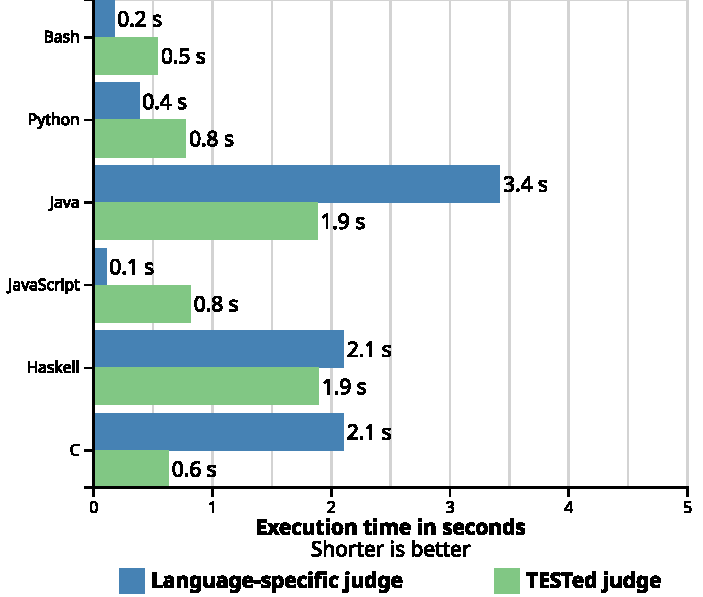
\includegraphics[width=0.8\textwidth]{performance}
    \caption{Runtime performance of TESTed versus language-specific test frameworks. For each programming language, we evaluated a correct submission for the same exercise with a language specific test framework and with TESTed.}
    \label{fig:performance}
\end{figure}

Our performance analysis indicates that an evaluation by TESTed is slower for Bash, Python and JavaScript.
This does not come as a surprise, since TESTed needs to do additional work in generating test code in the programming language of the submission and in serializing the results after executing the test code.
In addition, there are also differences in what evaluations are performed.
For example, the JavaScript judge does not lint submissions where TESTed systematically applies linting for all supported languages.
However, evaluations by TESTed are faster for Java, Haskell and C\@.
This is mainly due to implementation differences in the test frameworks, especially in the compilation step.
In TESTed, we have implemented the compilation step (and code generation) with as little overhead as possible, which is not always possible in language-specific judges.
For example, the Java framework relies on jUnit, while TESTed does not have any Java dependencies.

Performance remains a focus area for future work.
Automated test frameworks often deliver just-in-time feedback and are integrated into highly interactive learning environments.
As a result, students who frequently submit solutions during hands-on sessions or while working on homework assignments expect immediate results and get frustrated by poor response times.
Performance is therefore critical in educational software testing.
When implementing TESTed, we paid specific attention to reduce overhead during test code generation, compilation and execution, for example by bundling multiple contexts in a single compilation and execution step, making the performance of TESTed acceptable.
However, conditions in which TESTed may bundle contexts could still be improved, so that more contexts from the same test suite could be compiled and executed together.
Since test code generation only depends on a test suite and a selected programming language, we might also consider caching as a way to reuse generated test code for all submissions of a programming exercise that share the same programming language.
Performance could also be boosted by linting submissions in parallel to testing them, where TESTed currently runs these two steps sequentially.

\section{Conclusion}\label{sec:tested1-conclusion}

Educational software testing is the application of test frameworks to provide automated feedback on solutions that students submit for programming exercises.
We identified output comparison and unit testing as two opposing strategies commonly used in educational practice, and investigated the impact of both approaches on programming language support of the frameworks.
Test frameworks adopting unit testing enable fine-grained software testing, but are highly language specific.
The output comparison approach, on the other hand, is more generic in that it supports multiple programming languages, but imposes severe restrictions on programming exercises, granularity of testing and quality of feedback.

Our goal was to combine the best of both worlds.
We formulated requirements for programming-language-agnostic test frameworks that combine unit testing with support for multiple programming languages.
We see three clear benefits for the adoption of such frameworks.
First, exercise designers only need to know and use a single test framework to create programming exercises with support for automated feedback, irrespective of the target programming language, instead of switching to a new test framework for each programming language, taking into account restrictions on what can be tested or giving up on the quality of feedback.
Second, programming exercises only need a single test suite to evaluate solutions in a multitude of programming languages.
This allows teachers to reuse the same programming exercise for a language of their choice or to give students the freedom to solve exercises in their preferred language.
Third, it also saves time and effort to support educational software testing for new programming languages as common functionality of test frameworks is implemented once in a generic way, and only needs to be complemented with a thin layer of language specific configurations for each individual programming language.

To validate the feasibility of designing programming-language-agnostic test frameworks, we implemented a proof-of-concept framework called TESTed.
Having such a prototype also enabled us to evaluate the framework in educational practice.
The realization of TESTed confirms that the requirements for programming-language-agnostic test frameworks can be met and provides a framework that can be used in educational practice.
At the same time, working on and with TESTed also brought forward some areas for improvement and further research.

\end{document}
